\documentclass{article}

\usepackage{tikz}
\usepackage{tikz-network}

\begin{document}
    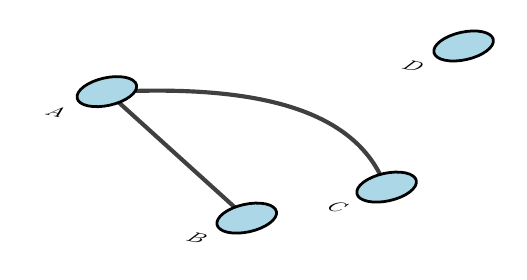
\begin{tikzpicture}[multilayer=3d]
        \Vertex[label=A,position=below,layer=1]{A}
        \Vertex[label=D,position=below,layer=1, x=3, y=2]{D}
        \Vertex[label=B,position=below,y=1,x=1,layer=2]{B}
        \Vertex[label=C,position=below,y=2,x=2,layer=2]{C}
        \Edge(A)(B)
        \Edge[bend=30](A)(C)
    \end{tikzpicture}
    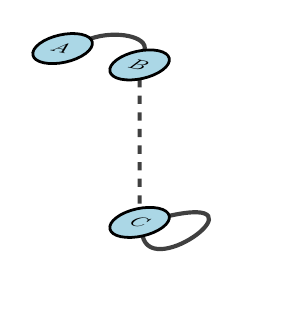
\begin{tikzpicture}[multilayer=3d]
        \Vertex[x=0.5,IdAsLabel,layer=1]{A}
        \Vertex[x=1.5,IdAsLabel,layer=1]{B}
        \Vertex[x=1.5,IdAsLabel,layer=2]{C}
        \Edge[bend=60](A)(B)
        \Edge[style=dashed](B)(C)
        \Edge(C)(C)
    \end{tikzpicture}
\end{document}

